%%%%%%%%%%%%%%%%%%%%%%%%%%%%%%%%%%%%%%%%%%%%%%%%%%%%%%%%%%%%%%%%%%%%%%%%%%%%%%
%
% Section file included in main project file using \input{}
%
% Assumes that LaTeX2e macros and packages defined in cg_comp.sty are
%   available
%
%%%%%%%%%%%%%%%%%%%%%%%%%%%%%%%%%%%%%%%%%%%%%%%%%%%%%%%%%%%%%%%%%%%%%%%%%%%%%%

 \section{Introduction and Background\label{sct:intro}}

Any musician who has wrestled with the temperament of a fretted stringed instrument is well aware of the challenges presented by tuning and pitch. In addition to the mathematical physics of musical scales~\cite{ref:durfee2015pms}, the mechanical specifications of the instrument and the strings themselves~\cite{ref:morse1981vas,ref:fletcher2005pmi} require accommodation during both manufacturing~\cite{ref:byers1996cgi,ref:varieschi2010icf} and tuning to achieve harmonious results. We can gain an appreciation for this problem by analyzing the expression for the allowed vibration frequencies of an ideal string, given by~\cite{ref:morse1981vsa,ref:fletcher2005pma}
 \begin{equation} \label{eqn:f_0_def}
f_q = \frac{q}{2\, L_0}\, \sqrt{\frac{T_0}{\mu_0}}\, ,
 \end{equation}
where $q \in \mathbb{N} = \{1, 2, \dots\}$, $L_0$ is the length of the free (unfretted) string from the saddle to the nut, $T_0$ is the tension in the free string, and $\mu_0 \equiv M / L_0$ is the linear mass density of a free string of mass $M$. The act of fretting the string changes its length, and therefore its frequency. For example, modern classical guitars are manufactured with frets placed along the fretboard using the Twelve-Tone Equal Temperament (12-TET) system, whereby the resonant length of a string pressed behind fret $n$ ideally should be $L_0 2^{-n/12}$, thereby producing a note with frequency $f_1 2^{n/12}$. But this result can never be achieved perfectly in reality. First, the string is elevated above the frets by the saddle and nut, so the fretted string is slightly elongated relative to the free string, and the resulting frequency is flattened in pitch. In principle, this effect could be accommodated by minute changes in the positions of the frets, but there are additional practical complications. For example, the string's tension and density are altered by the change in length, causing the frequency to sharpen by an amount that significantly exceeds the reduction caused by the increase in the resonant string length. In addition, the string is by no means ideal, and its intrinsic stiffness results in an additional increase in pitch that depends on its mechanical characteristics. These guitar intonation difficulties seem to preclude successful temperament, but remarkably the instrument can be \emph{compensated} by moving the positions of the saddle and the nut by small distances during the manufacturing process. Our goal in this work is to build an intuitive understanding of these effects to aid in the compensation and subsequent tuning of the classical guitar.

Throughout this work, we will use \emph{cents} to describe small differences in pitch~\cite{ref:durfee2015pms}. One cent is one one-hundredth of a 12-TET half-step, so that there are 1200~cents per octave. An experienced guitar player can distinguish beat notes with a difference frequency of $\Delta f \approx 1$~Hz, which corresponds to 8~cents at $A_3$ ($f = 220$~Hz) or 5~cents at $E_4$ ($f = 329.63$~Hz). Using this approach, the difference in pitch between two frequencies $f_1$ and $f_2$ is defined as
 \begin{equation} \label{eqn:cents_def}
\Delta \nu \equiv 1200\, \log_2\left(\frac{f_2}{f_1}\right)\, .
 \end{equation}
We define the average frequency $f \equiv (f_1 + f_2) / 2$ and the frequency difference $\Delta f \equiv f_2 - f_1$. Then
 \begin{equation} \label{eqn:cents_approx}
\Delta \nu = 1200\, \log_2\left(\frac{f + \Delta f / 2}{f - \Delta f /2}\right) \approx \frac{1200}{\ln 2}\, \frac{\Delta f}{f}\, ,
 \end{equation}
where the last approximation applies when $\Delta f \ll f$. As shown in \fig{diff_pitch}, if the average frequency of the interval is used to compute $f$ --- rather than the initial frequency $f_1$ --- then the accuracy of \eqn{cents_approx} holds for almost an entire octave. In this plot, we chose $f_1 = A_3 = 220$~Hz, and allowed $f_2$ to vary from $A_3$ to $A_4 + 30 \textrm{ Hz} = 450$~Hz. At the octave, the error in $\Delta \nu$ arising from \eqn{cents_approx} is -46~cents, or $-4$\%. We compare two different definitions of $f$ in \eqn{cents_approx}: the average of $f_1$ and $f_2$, and simply $f = f_1$. Using the average frequency leads to a significantly better approximation.

\begin{figure}
    \centering
    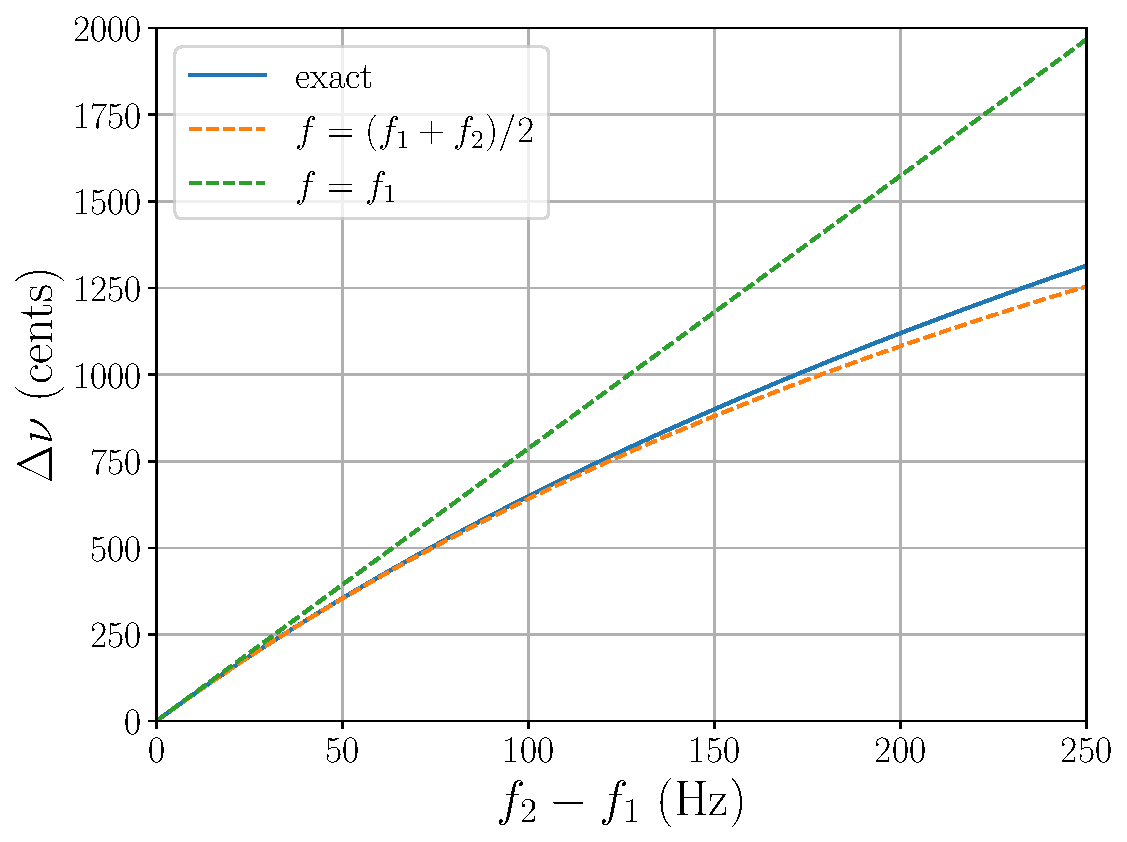
\includegraphics[width=6.5in]{../figures/diff_pitch}
    \caption{\label{fig:diff_pitch} Plot of $\Delta \nu$ for $f_1 = A_3 = 220$~Hz and $f_2$ varying from $A_3$ to $A_4 + 30 \textrm{ Hz} = 450$~Hz. We compare two different definitions of $f$ in \eqn{cents_approx}: the average of $f_1$ and $f_2$, and simply $f = f_1$. Using the average frequency leads to a significantly better approximation.}
\end{figure}
  

We present the basics of our model of classical guitar strings in \sct{model}, following the pioneering work of G.\ Byers~\cite{ref:byers1996cgi,ref:byersweb}. We begin with a new expression for the allowed vibration frequencies of a stiff string, derived in \app{freq} under the assumption that the boundary conditions at the saddle and the nut are not symmetric. We then include a discussion of the four contributions to frequency shifts and errors of non-ideal strings pressed behind a fret: the change in the resonant length of the string; a decrease in the linear mass density and an increase in the tension of the string; and the mechanical stiffness of the resonating string. Our goal is to simplify the equations through Taylor series expansions to allow an intuitive picture of the string's behavior to emerge. We offer an empirical reason to doubt the need for a complicated model of string fretting, and we explore this argument in greater detail in \app{fret}. In \sct{exp}, we suggest a simple experiment to estimate the response of the string's tension to the change in length caused by fretting, and we demonstrate the idea using a normal-tension string set on an Alhambra 8P guitar (as well as other string sets in \app{specs}). Then, in \sct{comp}, we use these estimates to demonstrate a straightforward analytic approach to compensating the errors in a guitar string, relying on a method --- described in \app{rms} --- to minimize the root-mean-squared (RMS) frequency deviation at each fret. Finally, in \sct{temp} we discuss a collaboration of guitar manufacturer and musician to temper the guitar using harmonic tuning and optimize it for a particular piece.

This document -- as well as the Python computer code needed to reproduce the figures -- is available at GitHub~\cite{ref:github2021rgb}. 